\documentclass[uplatex,dvipdfmx,a4paper,11pt]{jsreport}

\usepackage{docmute}


% 数式
\usepackage{amsmath,amsthm,amssymb}
\usepackage{bm}
% 画像
\usepackage{graphicx}

\usepackage{multirow}
\usepackage{wrapfig}
\usepackage{ascmac}
\usepackage{xcolor}


\usepackage{makeidx}
\makeindex

\graphicspath{{../../_Figures//}{../../_Figures/Rheology/}}

\usepackage{qrcode}
\setlength\lineskiplimit{0pt}
\setlength\normallineskiplimit{0pt}

\usepackage{qexam}

\usepackage{titlesec}
\titleformat*{\section}{\Large\bfseries}
\titleformat*{\subsection}{\large\bfseries}
\titleformat*{\subsubsection}{\normalsize\bfseries}
\titleformat*{\paragraph}{\normalsize\bfseries}

% ページ設定
% \pagestyle{empty}
% 高さの設定
\setlength{\textheight}{\paperheight}   % ひとまず紙面を本文領域に
\setlength{\topmargin}{-5.4truemm}      % 上の余白を20mm(=1inch-5.4mm)に
\addtolength{\topmargin}{-\headheight}  % 
\addtolength{\topmargin}{-\headsep}     % ヘッダの分だけ本文領域を移動させる
\addtolength{\textheight}{-40truemm}    % 下の余白も20mmに%% 幅の設定
\setlength{\textwidth}{\paperwidth}     % ひとまず紙面を本文領域に
\setlength{\oddsidemargin}{-5.4truemm}  % 左の余白を20mm(=1inch-5.4mm)に
\setlength{\evensidemargin}{-5.4truemm} % 
\addtolength{\textwidth}{-40truemm}     % 右の余白も20mmに
% 図と本文との間
%\abovecaptionskip=-5pt
%\belowcaptionskip=-5pt
%
% 全体の行間調整
% \renewcommand{\baselinestretch}{1.0} 
% 図と表
%\renewcommand{\figurename}{Fig.}
%\renewcommand{\tablename}{Tab.}
%

% \makeatletter 
% \def\section{\@startsection {section}{1}{\z@}{1.5 ex plus 2ex minus -.2ex}{0.5 ex plus .2ex}{\large\bf}}
% \def\subsection{\@startsection{subsection}{2}{\z@}{0.2\Cvs \@plus.5\Cdp \@minus.2\Cdp}{0.1\Cvs \@plus.3\Cdp}{\reset@font\normalsize\bfseries}}
% \makeatother 

\usepackage[dvipdfmx,%
 bookmarks=true,%
 bookmarksnumbered=true,%
 colorlinks=false,%
 setpagesize=false,%
 pdftitle={数式に頼らない直感的理解による材料設計のためのレオロジー⼊⾨},%
 pdfauthor={佐々木裕},%
 pdfsubject={},%
 pdfkeywords={レオロジー; 材料設計; }]{hyperref}
\usepackage{pxjahyper}

\usepackage{plext}

\usepackage{niceframe} 
\usepackage{framed}
\newenvironment{longartdeco}{%
  \def\FrameCommand{\fboxsep=\FrameSep \artdecoframe}%
  \MakeFramed {\FrameRestore}}%
 {\endMakeFramed}
 
\usepackage{siunitx}

\newcommand{\rmd}{\mathrm{d}}

\renewcommand{\questionFormat}[1]{
  \begin{center}{\textbf{\large{#1}}}\end{center}
}

\title{第1講 レオロジーのはじめの一歩\\演習問題}
\author{}
\date{}

\pagestyle{empty}

\begin{document}

\maketitle

\section*{第一章 「レオロジーとは」について (本文 $5\sim15$ p)}
\documentclass[uplatex,dvipdfmx,a4paper,11pt]{jsarticle}

\usepackage{docmute}


% 数式
\usepackage{amsmath,amsthm,amssymb}
\usepackage{bm}
% 画像
\usepackage{graphicx}

\usepackage{multirow}
\usepackage{wrapfig}
\usepackage{ascmac}
\usepackage{xcolor}


\usepackage{makeidx}
\makeindex

\graphicspath{{../../_Figures//}{../../_Figures/Rheology/}}

\usepackage{qrcode}
\setlength\lineskiplimit{0pt}
\setlength\normallineskiplimit{0pt}

\usepackage{qexam}

\usepackage{titlesec}
\titleformat*{\section}{\Large\bfseries}
\titleformat*{\subsection}{\large\bfseries}
\titleformat*{\subsubsection}{\normalsize\bfseries}
\titleformat*{\paragraph}{\normalsize\bfseries}

% ページ設定
% \pagestyle{empty}
% 高さの設定
\setlength{\textheight}{\paperheight}   % ひとまず紙面を本文領域に
\setlength{\topmargin}{-5.4truemm}      % 上の余白を20mm(=1inch-5.4mm)に
\addtolength{\topmargin}{-\headheight}  % 
\addtolength{\topmargin}{-\headsep}     % ヘッダの分だけ本文領域を移動させる
\addtolength{\textheight}{-40truemm}    % 下の余白も20mmに%% 幅の設定
\setlength{\textwidth}{\paperwidth}     % ひとまず紙面を本文領域に
\setlength{\oddsidemargin}{-5.4truemm}  % 左の余白を20mm(=1inch-5.4mm)に
\setlength{\evensidemargin}{-5.4truemm} % 
\addtolength{\textwidth}{-40truemm}     % 右の余白も20mmに
% 図と本文との間
%\abovecaptionskip=-5pt
%\belowcaptionskip=-5pt
%
% 全体の行間調整
% \renewcommand{\baselinestretch}{1.0} 
% 図と表
%\renewcommand{\figurename}{Fig.}
%\renewcommand{\tablename}{Tab.}
%

% \makeatletter 
% \def\section{\@startsection {section}{1}{\z@}{1.5 ex plus 2ex minus -.2ex}{0.5 ex plus .2ex}{\large\bf}}
% \def\subsection{\@startsection{subsection}{2}{\z@}{0.2\Cvs \@plus.5\Cdp \@minus.2\Cdp}{0.1\Cvs \@plus.3\Cdp}{\reset@font\normalsize\bfseries}}
% \makeatother 

\usepackage[dvipdfmx,%
 bookmarks=true,%
 bookmarksnumbered=true,%
 colorlinks=false,%
 setpagesize=false,%
 pdftitle={数式に頼らない直感的理解による材料設計のためのレオロジー⼊⾨},%
 pdfauthor={佐々木裕},%
 pdfsubject={},%
 pdfkeywords={レオロジー; 材料設計; }]{hyperref}
\usepackage{pxjahyper}

\usepackage{plext}

\usepackage{niceframe} 
\usepackage{framed}
\newenvironment{longartdeco}{%
  \def\FrameCommand{\fboxsep=\FrameSep \artdecoframe}%
  \MakeFramed {\FrameRestore}}%
 {\endMakeFramed}
 
\usepackage{siunitx}

\newcommand{\rmd}{\mathrm{d}}

\usepackage[inline]{showlabels}

\begin{document}

\question{演習問題 1}
内容を振り返るために、以下に示した文章例の中から適切な記述のものを複数選んでください。
\begin{qlist}
	\qitem レオロジーとはどのようなものでしょうか?
		\begin{qlist2}
			\qitem レオロジーとは「物質の変形と流動に関する科学」であり、これまでの物理理論とはかけ離れた新規な測定技術です。
			\qitem レオロジーのベースとなる物体の変形や流動に関する物理学は、古くから弾性論や流体論として存在していました。
			\qitem 弾性論はフックの法則を基本にして弾性固体の力学的な性質を記述し、流体論はニュートンの法則により粘性を持つ流体の流れ方の挙動を明確にします。
			\qitem レオロジー測定は、物質の変形や流動を測って、そこに加えられた刺激を推定する逆問題を解きます。
			\qitem レオロジー測定を通して、物質の持つ各種の特性を比較することができるようになります。
    \end{qlist2}
    \vspace{3mm}
	\qitem 会社の仕事とレオロジーとの関係について確認してみましょう。
		\begin{qlist2}
			\qitem レオロジーという学問は高度に学際的な科学であり、同時に、それぞれの要素技術が大きく異る多岐にわたる対象を多様な切り口で議論していきます。
			\qitem レオロジーは、物質の特性を絶対値として測定する方法で、物質に含有される成分を定量的に分析することができます。
			\qitem 商品の開発の「原料から材料そして商品へと仕立てる過程」において、特性の評価にレオロジーを活用することができます。
            \qitem 例えば、人間の心地良さの定量化や、原料、材料の機能設計にレオロジーが活用されている事例が多くあります。
            \qitem 人間の感覚のような抽象的なものは定量化する方法がありませんから、できるだけ過去の記憶や勘を働かせることで設計を進めるしかありません。
    \end{qlist2}
    \vspace{3mm}
	\qitem 人がもっている感覚とレオロジーとはどのような関係があるのでしょうか?
		\begin{qlist2}
            \qitem オノマトペとは様々な状態や感情を言葉に表したものであり、レオロジー的な違いを定性的に表現できます。
            \qitem 人間は身の回りにある様々な状態や感情に言葉を与えますが、そのような定性的な評価はレオロジーとは関係ありません。
			\qitem 人間は、ものを叩いたり触ったりして刺激を与えて、その応答を音で聞いたり手触りで感じることで、レオロジー評価を行う事ができます。
			\qitem 人間のレオロジー的な感覚を表現したウェーバー・フェヒナーの法則があり、基準とする値に応じて違いを見極める閾値が変わります。
            \qitem 人間の感覚は強い刺激の変化にとても敏感で、絶対的な差を感じることができます。
    \end{qlist2}
    \vspace{3mm}
	\qitem レオロジーを理解するために考えるべきことは?
		\begin{qlist2}
			\qitem 人間は手触りでレオロジー的な違いを判断できますが、定量的な評価を判断することはあまりうまくできません。
            \qitem 感覚的な違いを言葉で表せば、十分に人に伝わる定量的な評価になります。
            \qitem 以前に実施した実験の結果は実験事実なのだから、その内容の整合性など考えることなく過去の知見として使っていけます。
			\qitem 著者のおすすめは、標語的には「急がば回れ」であり、慌てずに、イメージとして全体像をザックリと捕まえることができれば、理解は一気に容易になると期待しています。
			\qitem 会社の仕事として命令されたような事項であっても、「何のためにやりたいのか」という目的と「何をやりたいのか」という目標をきちんと設定することが最も大事になります。
		\end{qlist2}
\end{qlist}

\question{演習問題 2}
内容を振り返るために、テキストで用いた言葉を使って簡単な穴埋めを行ってください。

\begin{qparts}
    \qpart 「レオロジーとは」について、以下の\qbox{(a)}から\qbox{(i)}までのカッコを埋めてください。
    \begin{qlist}
      \qitem レオロジーとは「物質の\qbox{}に関する科学」であり、既存の弾性論や流体論をベースとして、物質の持つ各種の特性を比較することができる学問です。
      決して新規な\qbox{}ではなく、過去の\qbox{}を利用していく必要があります。
      \qitem レオロジーの対象は多岐にわたりますが、基本的に物質の特性を\qbox{}する技術であり、\qbox{}が主となります。
      \qitem 人間のレオロジー的な能力はとても高く、様々な違いを定性的に感じることができます。ただし、その\qbox{}に感じるだけであり、また、基準に応じて\qbox{}することを理解する必要があります。
      \qitem レオロジーが相対的な比較であることをきちんと理解して、落ち着いて\qbox{}で議論しましょう。また、\qbox{}を明確にすることはとても大事です。
    \end{qlist}

    \begin{itembox}[l]{選択肢}
      \begin{center}
        \begin{tabular}{lllll}
                1. 目的と目標&2. 差を相対的に&3. 相対的に比較&4. 定性的な評価 & 5. 閾値が変化 \\
                6. 変形と流動&7. 多様な知見&8. わかり易い言葉 & 9. 測定技術
        \end{tabular}
      \end{center}
    \end{itembox}
\end{qparts}

\question{演習問題 3}
\begin{qparts}
    \qpart 「何をなんのためにやりたいのか」という目的や目標は皆さんそれぞれのものをお持ちであり、そのためにレオロジーを学ばれているのだと思います。
    折角の機会ですから、一度ご自身の有りたい姿について考えをまとめてみてはいかがでしょうか。

    以下に、かんたんに設問の形で項目を上げてみました。
    \vspace{-2mm}
    \begin{qlist}
        \qitem ご自分の仕事を、全く事前の知識を持たない他の人にでも理解できるように説明してみましょう。
        \qitem その仕事の中での、ご自分の役割をシンプルに表現してみてください。
        \qitem ご自分の役割の中で、何をやらなくてはいけないと感じていますか?
        \qitem その使命は、何のためにやっているのでしょうか?
        \qitem 上述の状態の中で、レオロジーにはどのようなことを期待していますか?
    \end{qlist}
    \vspace{-2mm}
    \qpart もしもご相談されたいことがあれば、書いていただければ相談に乗ります。(なお、こちらは提出は義務ではありません。)
\end{qparts}

\end{document}
\clearpage
\section*{第一章 「レオロジーとは」について (本文 $5\sim15$ p)}
\begin{document}

\question{解答欄 1}
\begin{table}[htb]
    \begin{center} 
      \begin{tabular}{|p{.15\textwidth}|p{.15\textwidth}|p{.15\textwidth}|p{.15\textwidth}|p{.15\textwidth}|} \hline
        (1) & (2) & (3) & (4) & (5)\\ \hline \hline
          &  & & &  \\ \hline		
      \end{tabular}
    \end{center}
  \end{table}

  \question{解答欄 2}
  \begin{table}[htb]
    \begin{center} 
      \begin{tabular}{|p{.08\textwidth}|p{.08\textwidth}|p{.08\textwidth}|p{.08\textwidth}|p{.08\textwidth}|p{.08\textwidth}|p{.08\textwidth}|p{.08\textwidth}|p{.08\textwidth}|} \hline
        (a) & (b) & (c) & (d) & (e) & (f) & (g) & (h) & (i)\\ \hline
          &  & & & & & & &  \\ \hline		
      \end{tabular}
    \end{center}
  \end{table}

  \question{解答欄 3}
    \begin{table}[htb]
    \renewcommand\arraystretch{3.0}
    \begin{center} 
      \begin{tabular}{|c|p{.8\textwidth}|} \hline
        (1) & \\ \hline
        (2)  & \\ \hline
        (3) & \\ \hline
        (4)  & \\ \hline
        (5) & \\ \hline
        自由  & \\ \hline
      \end{tabular}
    \end{center}
  \end{table}

\end{document}

\clearpage
\section*{第二章 「レオロジーを始める前に」について (本文 $17\sim25$ p)}
\documentclass[uplatex,dvipdfmx,a4paper,11pt]{jsarticle}

\usepackage{docmute}


% 数式
\usepackage{amsmath,amsthm,amssymb}
\usepackage{bm}
% 画像
\usepackage{graphicx}

\usepackage{multirow}
\usepackage{wrapfig}
\usepackage{ascmac}
\usepackage{xcolor}


\usepackage{makeidx}
\makeindex

\graphicspath{{../../_Figures//}{../../_Figures/Rheology/}}

\usepackage{qrcode}
\setlength\lineskiplimit{0pt}
\setlength\normallineskiplimit{0pt}

\usepackage{qexam}

\usepackage{titlesec}
\titleformat*{\section}{\Large\bfseries}
\titleformat*{\subsection}{\large\bfseries}
\titleformat*{\subsubsection}{\normalsize\bfseries}
\titleformat*{\paragraph}{\normalsize\bfseries}

% ページ設定
% \pagestyle{empty}
% 高さの設定
\setlength{\textheight}{\paperheight}   % ひとまず紙面を本文領域に
\setlength{\topmargin}{-5.4truemm}      % 上の余白を20mm(=1inch-5.4mm)に
\addtolength{\topmargin}{-\headheight}  % 
\addtolength{\topmargin}{-\headsep}     % ヘッダの分だけ本文領域を移動させる
\addtolength{\textheight}{-40truemm}    % 下の余白も20mmに%% 幅の設定
\setlength{\textwidth}{\paperwidth}     % ひとまず紙面を本文領域に
\setlength{\oddsidemargin}{-5.4truemm}  % 左の余白を20mm(=1inch-5.4mm)に
\setlength{\evensidemargin}{-5.4truemm} % 
\addtolength{\textwidth}{-40truemm}     % 右の余白も20mmに
% 図と本文との間
%\abovecaptionskip=-5pt
%\belowcaptionskip=-5pt
%
% 全体の行間調整
% \renewcommand{\baselinestretch}{1.0} 
% 図と表
%\renewcommand{\figurename}{Fig.}
%\renewcommand{\tablename}{Tab.}
%

% \makeatletter 
% \def\section{\@startsection {section}{1}{\z@}{1.5 ex plus 2ex minus -.2ex}{0.5 ex plus .2ex}{\large\bf}}
% \def\subsection{\@startsection{subsection}{2}{\z@}{0.2\Cvs \@plus.5\Cdp \@minus.2\Cdp}{0.1\Cvs \@plus.3\Cdp}{\reset@font\normalsize\bfseries}}
% \makeatother 

\usepackage[dvipdfmx,%
 bookmarks=true,%
 bookmarksnumbered=true,%
 colorlinks=false,%
 setpagesize=false,%
 pdftitle={数式に頼らない直感的理解による材料設計のためのレオロジー⼊⾨},%
 pdfauthor={佐々木裕},%
 pdfsubject={},%
 pdfkeywords={レオロジー; 材料設計; }]{hyperref}
\usepackage{pxjahyper}

\usepackage{plext}

\usepackage{niceframe} 
\usepackage{framed}
\newenvironment{longartdeco}{%
  \def\FrameCommand{\fboxsep=\FrameSep \artdecoframe}%
  \MakeFramed {\FrameRestore}}%
 {\endMakeFramed}
 
\usepackage{siunitx}

\newcommand{\rmd}{\mathrm{d}}

\usepackage[inline]{showlabels}

\begin{document}

\question{演習問題 1}
内容を振り返るために、以下に示した文章例の中から適切な記述のものを複数選んでください。
\begin{qlist}
	\qitem 「関数」と「グラフ」というそれぞれの考え方を表す正しい言葉はどれでしょうか?
		\begin{qlist2}
			\qitem 関数とは、入力と出力との間の関係を表している変換装置のようなものと捉えられます。
			\qitem 関数とは、数の集合に値を取る写像の一種です。
			\qitem 関数とは、ものの関係を表す数のことを指します。
			\qitem グラフとは、入力と出力との関係を視覚的に理解しやすくしたものです。
			\qitem グラフを用いることで、関数の出力の値を正確に読み取ることができます。
		\end{qlist2}
    \vspace{3mm}
	\qitem 「線型性」と「物理モデル」というそれぞれの考え方を表す正しい言葉はどれでしょうか?
		\begin{qlist2}
			\qitem 線型性とは、グラフに表した時に原点を通る直線となるような性質であり、比例の関係を表します。
			\qitem 線型性とは、放物線と呼ばれる曲線で表される性質であり、反比例の関係を表します。
			\qitem 物理モデルとは、「事象や理論の成り立ちを説明するための簡単で理解しやすい概念や模型」です。
			\qitem 我々の身の回りに起こっている実際の事柄は、非常に単純で線型で記述できる場合がほとんどです。
			\qitem 入力が小さい場合には応答が線型で取り扱える場合が多いことが知られています。
    \end{qlist2}
    \vspace{3mm}
	\qitem 「量」について正しい記述を選んでください。
		\begin{qlist2}
			\qitem 量とは、定性的に区別でき、かつ、定量的に決定できるものです。
			\qitem 同じ種類の量同士は「和と差」の演算が定義できて、結果は同じ種類の量となります。
			\qitem 異なる種類の量であっても、いかなる演算でもできます。
			\qitem 同じ、あるいは、異なる種類の量同士でも積や商が定義できる場合もあります。
			\qitem 長さ同士の積は、体積を表します。
    \end{qlist2}
    \vspace{3mm}
	\qitem 「次元」について正しい記述を選んでください。
		\begin{qlist2}
			\qitem 次元とは、注目する「ある量」が、どのような現象であるかを「基本量の積と商で表す」ような考え方といえます。
			\qitem 面積という量は、長さという基本量が掛け合わされることで、広さという現象を表しています。
			\qitem 次元とは、物質の性質を表す量のことです。
			\qitem 次元の関係式とは「定数係数を無視した等式として表すことで物理現象の成り立ちを表して」います。
			\qitem ここで用いた次元という考え方は、一般に使われている三次元や四次元という言葉とは全く関係ありません。
		\end{qlist2}
    \vspace{3mm}
	\qitem 「単位」について正しい記述を選んでください。
		\begin{qlist2}
			\qitem 単位とは、「量の大きさを表すため」に特定の会社間で取り決めによって定義されたものです。
			\qitem 単位とは、「同種の物理量の大きさを表すため」に取り決めによって定義されたものです。
			\qitem 現在、最も広く使われている単位系は、国際単位系(SI)です。
			\qitem JIS と呼ばれる単位系は、日本で広く使われています。
			\qitem 任意の物理量の値 $Q$ は、その大きさを表す数値 $n$ と単位 $U$ との積として表されることになります。
		\end{qlist2}
\end{qlist}

\question{演習問題 2}
内容を振り返るために、テキストで用いた言葉を使って簡単な穴埋めを行ってください。
\begin{qlist}
  \qitem 量の次元に関して、国際量体系で表のように7つの基本量が定められています。レオロジーでよく使う四つの基本量を、
  以下の\qbox{(a)}から\qbox{(d)}までのカッコを埋めてください。
	\begin{center}
		\begin{tabular}{|c|c||c|c|} \hline
			基本量 		& 次元の記号 & SI単位 		& 単位の記号\\ \hline \hline
			\qbox{}		& L			& メートル 		& m \\ \hline
			\qbox{}		& M			& キログラム 	& kg \\ \hline
			\qbox{}		& T			& 秒 			& s \\ \hline
			電流		& I			& アンペア 		& A \\ \hline
			\qbox{}	& $\Theta$	& ケルビン 		& K \\ \hline
			物質量		& N			& モル 			& mol \\ \hline
			光度		& J			& カンデラ 		& cd \\ \hline
		\end{tabular}
	\end{center}

	\qitem 以下に示した組立単位について、以下の\qbox{(e)}から\qbox{(i)}までのカッコを埋めてください。
	\begin{center}
		\begin{tabular}{|c|c||c|c|} \hline
			組立量 		& 名称					& 記号		& SI 基本単位による表現 	\\ \hline \hline
			\qbox{}		& ヘルツ (hertz)		& Hz		&  s$^{-1}$ 					\\ \hline
			\qbox{}		& ニュートン (newton)	& N 		& m$\cdot$kg$\cdot$s$^{-2}$ 	\\ \hline
			\qbox{}		& パスカル (pascal)		& Pa 		& (N/m$^2$) = m$^{-1}\cdot$kg$\cdot$s$^{-2}$ \\ \hline
			\qbox{}	& ジュール (joule)		& J 		& (N$\cdot$m) = m$^{2}\cdot$kg$\cdot$s$^{-2}$ \\ \hline
			\qbox{}		& パスカル秒			& Pa$\cdot$s & m$^{-1}\cdot$kg$\cdot$s$^{-1}$ \\ \hline
		\end{tabular}
  \end{center}
  
  \begin{itembox}[l]{選択肢}
    \begin{center}
      \begin{tabular}{lllll}
        1. 応力&2. 質量&3. 時間&4. エネルギー&5. 粘度\\
        6. 周波数&7. 長さ&8. 熱力学温度&9. 力
      \end{tabular}
    \end{center}
  \end{itembox}
\end{qlist}

\question{演習問題 3}
数行程度の簡単な記述で構いませんので、以下の自由記述問題を考えてみてください。
\begin{qlist}
\qitem 「レオロジー」という考え方を理解して、多様な場面において使いこなすためには、
「モデル化」という考え方がとても大事だと筆者は強く感じています。\\
皆さんがモデル化ということに対して感じることを書いてみてください。
\end{qlist}

\end{document}
\clearpage
\section*{第二章 「レオロジーを始める前に」について (本文 $17\sim25$ p)}
\begin{document}

\question{解答欄 1}
\begin{table}[htb]
    \begin{center} 
      \begin{tabular}{|p{.15\textwidth}|p{.15\textwidth}|p{.15\textwidth}|p{.15\textwidth}|p{.15\textwidth}|} \hline
        (1) & (2) & (3) & (4) & (5)\\ \hline \hline
          &  & & &  \\ \hline		
      \end{tabular}
    \end{center}
  \end{table}

  \question{解答欄 2}
  \begin{table}[htb]
    \begin{center} 
      \begin{tabular}{|p{.08\textwidth}|p{.08\textwidth}|p{.08\textwidth}|p{.08\textwidth}|p{.08\textwidth}|p{.08\textwidth}|p{.08\textwidth}|p{.08\textwidth}|p{.08\textwidth}|} \hline
        (a) & (b) & (c) & (d) & (e) & (f) & (g) & (h) & (i)\\ \hline
          &  & & & & & & &  \\ \hline		
      \end{tabular}
    \end{center}
  \end{table}

\question{解答欄 3}
\begin{table}[htb]
  % \renewcommand\arraystretch{2.0}
  \begin{center} 
    \begin{tabular}{|l|p{.8\textwidth}|} \hline
      & \\
      私にとっての  & \\
      モデル化とは  & \\ 
      & \\ \hline
    \end{tabular}
  \end{center}
\end{table}

\end{document}

\clearpage
\section*{第三章 「レオロジーのはじめの一歩」について (本文 $27\sim36$ p)}
\documentclass[uplatex,dvipdfmx,a4paper,11pt]{jsarticle}

\usepackage{docmute}


% 数式
\usepackage{amsmath,amsthm,amssymb}
\usepackage{bm}
% 画像
\usepackage{graphicx}

\usepackage{multirow}
\usepackage{wrapfig}
\usepackage{ascmac}
\usepackage{xcolor}


\usepackage{makeidx}
\makeindex

\graphicspath{{../../_Figures//}{../../_Figures/Rheology/}}

\usepackage{qrcode}
\setlength\lineskiplimit{0pt}
\setlength\normallineskiplimit{0pt}

\usepackage{qexam}

\usepackage{titlesec}
\titleformat*{\section}{\Large\bfseries}
\titleformat*{\subsection}{\large\bfseries}
\titleformat*{\subsubsection}{\normalsize\bfseries}
\titleformat*{\paragraph}{\normalsize\bfseries}

% ページ設定
% \pagestyle{empty}
% 高さの設定
\setlength{\textheight}{\paperheight}   % ひとまず紙面を本文領域に
\setlength{\topmargin}{-5.4truemm}      % 上の余白を20mm(=1inch-5.4mm)に
\addtolength{\topmargin}{-\headheight}  % 
\addtolength{\topmargin}{-\headsep}     % ヘッダの分だけ本文領域を移動させる
\addtolength{\textheight}{-40truemm}    % 下の余白も20mmに%% 幅の設定
\setlength{\textwidth}{\paperwidth}     % ひとまず紙面を本文領域に
\setlength{\oddsidemargin}{-5.4truemm}  % 左の余白を20mm(=1inch-5.4mm)に
\setlength{\evensidemargin}{-5.4truemm} % 
\addtolength{\textwidth}{-40truemm}     % 右の余白も20mmに
% 図と本文との間
%\abovecaptionskip=-5pt
%\belowcaptionskip=-5pt
%
% 全体の行間調整
% \renewcommand{\baselinestretch}{1.0} 
% 図と表
%\renewcommand{\figurename}{Fig.}
%\renewcommand{\tablename}{Tab.}
%

% \makeatletter 
% \def\section{\@startsection {section}{1}{\z@}{1.5 ex plus 2ex minus -.2ex}{0.5 ex plus .2ex}{\large\bf}}
% \def\subsection{\@startsection{subsection}{2}{\z@}{0.2\Cvs \@plus.5\Cdp \@minus.2\Cdp}{0.1\Cvs \@plus.3\Cdp}{\reset@font\normalsize\bfseries}}
% \makeatother 

\usepackage[dvipdfmx,%
 bookmarks=true,%
 bookmarksnumbered=true,%
 colorlinks=false,%
 setpagesize=false,%
 pdftitle={数式に頼らない直感的理解による材料設計のためのレオロジー⼊⾨},%
 pdfauthor={佐々木裕},%
 pdfsubject={},%
 pdfkeywords={レオロジー; 材料設計; }]{hyperref}
\usepackage{pxjahyper}

\usepackage{plext}

\usepackage{niceframe} 
\usepackage{framed}
\newenvironment{longartdeco}{%
  \def\FrameCommand{\fboxsep=\FrameSep \artdecoframe}%
  \MakeFramed {\FrameRestore}}%
 {\endMakeFramed}
 
\usepackage{siunitx}

\newcommand{\rmd}{\mathrm{d}}

\usepackage[inline]{showlabels}

\begin{document}

\question{演習問題 1}
内容を振り返るために、以下に示した文章例の中から適切な記述のものを複数選んでください。
	\begin{qlist}
		\qitem 力と釣り合いについての、正しい言葉はどれでしょうか?
		\begin{qlist2}
			\qitem 静力学とは、相互作用する物体系の運動について議論します。
			\qitem 物質に力を加えたとき、物質の内部には外力の何倍もの大きな力が生じます。
			\qitem 力とは、物体の状態を変化させる原因となる作用で、その作用の大きさを表す物理量と考えられます。
			\qitem 力の釣り合いを議論するものが静力学です。
			\qitem 作用した力と釣り合う力が生じることを、「作用・反作用の原理」といいます。
		\end{qlist2}
    \vspace{3mm}
	\qitem 「力学的な刺激と応答」についての、正しい言葉はどれでしょうか?
		\begin{qlist2}
			\qitem 物質に刺激を与えるということは変形させるということに対応し、変形の結果として応力という応答が生じます。
			\qitem ひずみとは、変形の状態を表す尺度であり、初期状態からどれだけ変位したかを表す無次元量です。
			\qitem ひずみとは、変形度合いを表す長さの次元を持った物理量です。
			\qitem 物質に加えた外力と応力とは、力の大きさを表す全く同一の物理量です。
			\qitem 応力の表す意味は単位面積あたりに働く内部の力ということになります。
		\end{qlist2}
    \vspace{3mm}
	\qitem 弾性体のモデルについての、正しい言葉はどれでしょうか?
		\begin{qlist2}
			\qitem 弾性体であっても、いったん外力により変形すると、もう元には戻りません。
			\qitem 弾性体はあたかもバネのように取り扱うことができます。
			\qitem 弾性体を表すモデルはニュートンの法則であり、ダッシュポットでイメージできます。
			\qitem 弾性体のフックモデルでは全体のひずみに比例するのは応力です。
			\qitem フックモデルでの比例定数が弾性率であり、応力と同じ次元 [Pa] です。
		\end{qlist2}
    \vspace{3mm}
	\qitem 「液体の変形と応答」についての、正しい言葉はどれでしょうか?
	\begin{qlist2}
		\qitem 液体は、「外力によって変形されたら元には戻れない」流れるという性質を持った物質です。
		\qitem 液体に変形を与えると流れ、変形を止めれば応力も消えます。
		\qitem いったん変形を加えると、液体内部での応力はずっと維持されます。
		\qitem 液体は、変形させる速度が変わると生じる応力も変わります。
		\qitem 水中ではゆっくり歩いても水の抵抗は変化しません。
	\end{qlist2}
  \vspace{3mm}
	\qitem 液体のモデルについての、正しい言葉はどれでしょうか?
	\begin{qlist2}
		\qitem 液体の流れるという性質は、ニュートンの法則で整理できます。
		\qitem 液体はせん断速度に反比例して流れやすさが低下します。
		\qitem せん断応力は、せん断速度に比例します。
		\qitem 物質の流れやすさを表す指標である粘度は、測定条件に応じて常に変化します。
		\qitem 液体の力学モデルは、ダッシュポットで表されます。
	\end{qlist2}
\end{qlist}

\question{演習問題 2}
内容を振り返るために、テキストで用いた言葉を使って簡単な穴埋めを行ってください。

\begin{qparts}
\qpart 「弾性体の力学的な刺激と応答」について、以下の\qbox{(a)}から\qbox{(i)}までのカッコを埋めてください。
		\begin{qlist}
			\qitem 変形は、物質を一つの軸に沿って引き伸ばす「\qbox{}」とトランプのカードを横にずらしたような「\qbox{}」の二つに単純化できます。
			\qitem 伸張変形では、\qbox{}を\qbox{}で除したものがひずみとなります。
			\qitem 応力とは、物質の内部に生じている\qbox{}を表す物理量であり、その表す意味は単位面積あたりの\qbox{}ということになります。
			\qitem 応力と力の関係は以下のように書けます。
			\begin{align*}
				\qbox{} = \dfrac{\qbox{}}{\qbox{}}
			\end{align*}
			% \qitem 一様な太さの棒を引っ張ったとき、棒の長手方向にはどの位置で切断したとしても、\qbox{}が働いていることに注意してください。

      \begin{itembox}[l]{選択肢}
        \begin{center}
          \begin{tabular}{lllll}
            1. 変形量	&2. せん断変形	&3. 力の大きさ	&4. 面積	&5. 応力\\
            6. 初期長さ	&7. 力		&8. 伸張変形				&9. 内部の力
          \end{tabular}
        \end{center}
      \end{itembox}

    \end{qlist}

\qpart 弾性体と液体の力学応答について、以下の\qbox{(j)}から\qbox{(p)}までのカッコを埋めてください。
		\begin{qlist}
			\qitem 弾性体を表すモデルはフックの法則であり、以下のように書けます。
				\begin{center}
					\begin{minipage}{0.45\textwidth}
						\begin{itemize}
							\item \qbox{} $\varepsilon$ と比例して、
							\item \qbox{} $\sigma$ が生じ、
							\item 比例定数が\qbox{} $E$
						\end{itemize}
						\begin{align*}
							\sigma = E \varepsilon
						\end{align*}
					\end{minipage}
					\begin{minipage}{0.35\textwidth}
						\begin{center}
						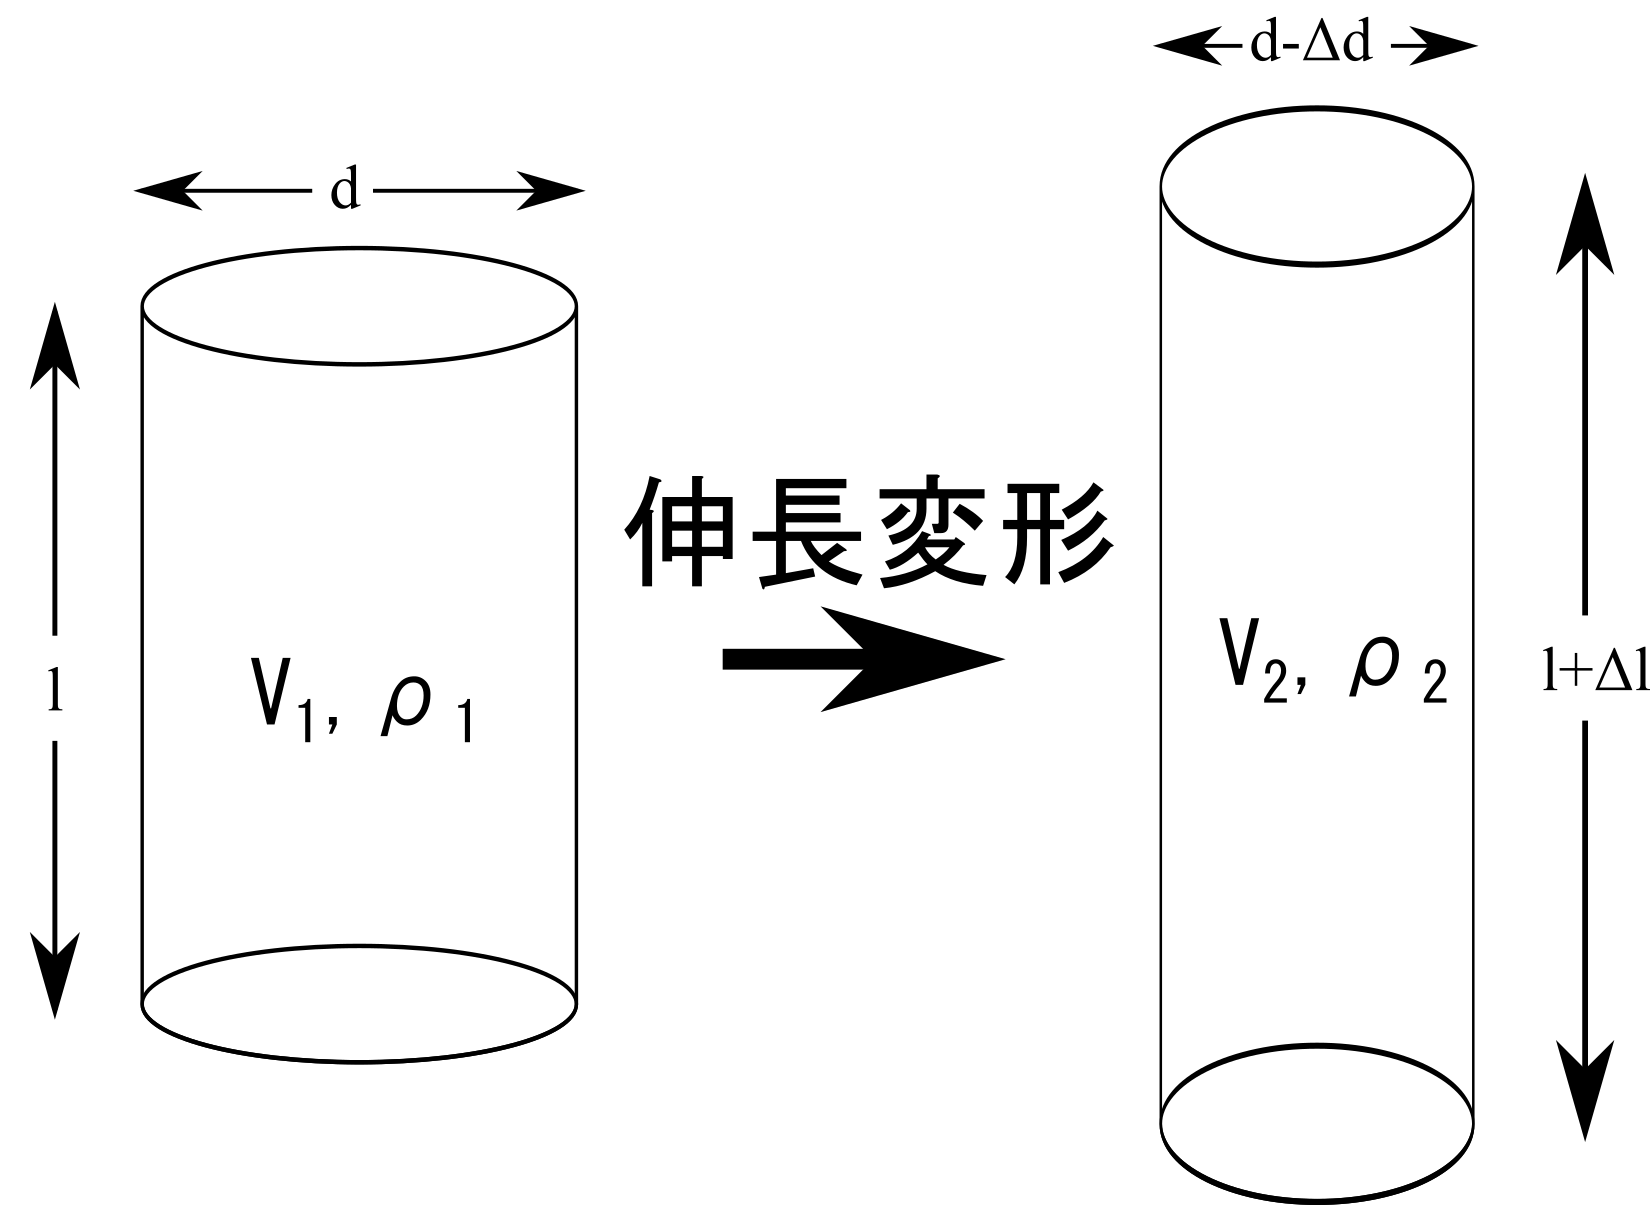
\includegraphics[width=.8\textwidth]{hook_law.png}
						\end{center}
					\end{minipage}
				\end{center}
			\qitem 液体の評価は主としてそのひずみ速度を維持しやすい「\qbox{}」により行われる場合が多くなります。
			\qitem ニュートンの法則の比例関係を式で表せば以下のようになります。
			\begin{align*}
				\text{\qbox{}} &= \text{\qbox{}} \times \text{\qbox{}} \notag \\
				\tau &= \eta \dot{\gamma}
      \end{align*}
      
      \begin{itembox}[l]{選択肢}
        \begin{center}
          \begin{tabular}{llll}
            1. 伸張弾性率	&2. ひずみ速度	&3. 伸張ひずみ	&4. せん断応力\\
            5. 伸張応力 	&6. せん断変形	&7. 粘度		
          \end{tabular}
        \end{center}
      \end{itembox}
  \end{qlist}

\end{qparts}

\question{演習問題 3}
数行程度の簡単な記述で構いませんので、以下の自由記述問題を考えてみてください。
\begin{qlist}
\qitem この章では、レオロジーのはじめの一歩として、その力学モデルについて簡単な説明を行ってきました。
弾性体と液体の力学モデルの特徴についてそれぞれ簡単にまとめて、その大きな違いについて書いてみてください。
\end{qlist}

\clearpage

\end{document}
\clearpage
\section*{第三章 「レオロジーのはじめの一歩」について (本文 $27\sim36$ p)}
\begin{document}

\question{解答欄 1}
\begin{table}[htb]
  \begin{center} 
    \begin{tabular}{|p{.15\textwidth}|p{.15\textwidth}|p{.15\textwidth}|p{.15\textwidth}|p{.15\textwidth}|} \hline
      (1) & (2) & (3) & (4) & (5)\\ \hline \hline
        &  & & &  \\ \hline		
    \end{tabular}
  \end{center}
\end{table}

  \question{解答欄 2}
  \begin{table}[htb]
    \begin{center} 
      \begin{tabular}{|p{.08\textwidth}|p{.08\textwidth}|p{.08\textwidth}|p{.08\textwidth}|p{.08\textwidth}|p{.08\textwidth}|p{.08\textwidth}|p{.08\textwidth}|} \hline
        (a) & (b) & (c) & (d) & (e) & (f) & (g) & (h)\\ \hline
          &  & & & & & &  \\ \hline		
          (i) & (j) & (k) & (l) & (m) & (n) & (o) & (p)\\ \hline
          &  & & & & & &  \\ \hline		
      \end{tabular}
    \end{center}
  \end{table}

\question{解答欄 3}
\begin{table}[htb]
  % \renewcommand\arraystretch{2.0}
  \begin{center} 
    \begin{tabular}{|l|p{.8\textwidth}|} \hline
      & \\
      弾性体と液体の  & \\
      力学モデルの違い  & \\ 
      & \\ \hline
    \end{tabular}
  \end{center}
\end{table}

\end{document}

\end{document}